\sys is a new programming and execution model for intermittent computing on energy-harvesting devices. \sys addresses the challenges outlined in Section~\ref{sec:background} to make task-based intermittent programs {\em accessible}, {\em efficient} and {\em flexible}. \sys accomplishes this goal with a constellation of a new programming model, compiler, and run time software system support, refer to Figure~\ref{fig:system_overview}.

\begin{figure}
	\centering
	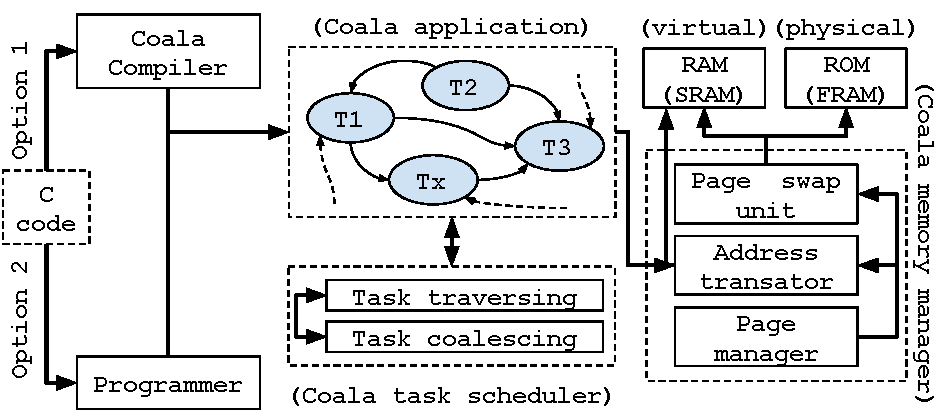
\includegraphics[width=\columnwidth]{figures/viper_block_diagram.pdf}
	\caption{\sys top-level view.}
	\label{fig:system_overview}
\end{figure}

\textbf{\sys Programming Model.} To use \sys, a programmer first writes plain, imperative C code. The programmer then has an option to {\em manually} or {\em automatically} translate the program into code for \sys's task-based programming model. To manually translate, the programmer decomposes the program into tasks, and annotates memory accesses that manipulate data shared by multiple tasks. To automatically translate, the programmer simply uses \sys's compiler (described in Section~\ref{sec:compiler}), which decomposes a program into tasks and annotates accesses to task-shared data. After translating to task-based code and compiling, the programmer has an executable \sys binary.

\sys's programming interface, listed in Table~\ref{tab:viper_syntax}, consists of
constructs for defining tasks~\cite{chain,alpaca} and accessors for
protected variables shared between tasks. These anotations are added either by
the programmer (in the manual translation mode) or the compiler (in automatic
translation mode). As in prior task-based intermittent programming
models~\cite{chain,alpaca}, tasks are functions that are not allowed to have
any direct callers but receive control by explicit {\tt next\_task} statements.
In \sys, a task transition atomically commits the memory operations of the
current task.  The programmer identifies each task by adding the {\tt task}
keyword to the function's declaration and designates one task as the {\em
origin} task at which execution begins. After a power failure,
\sys restarts from the last (partially) executed task.
%
A \sys program manipulates {\em protected} state---accessed by more than one
task---using the \emph{read variable} ({\tt RVAR}) and \emph{write variable}
({\tt WVAR}) operations. These operations convey to \sys's memory manager which
data must be buffered in volatile memory and committed.

\begin{table}
	\centering
	\footnotesize
	\begin{tabular}{|c|c|}
		\hline
		\textbf{Keyword} & \textbf{Description} \\
		\hline\hline
		\texttt{task foo() \{...\}} & Task definition\\
		\texttt{origin task foo() \{...\}} & Origin task definition\\
		\texttt{next\_task(t)} & Transition to task \texttt{t}\\
		\texttt{u = RVAR(v)} & Read protected variable \texttt{v} into \texttt{u}\\
		\texttt{WVAR(v, u)} & Write \texttt{u} to protected variable \texttt{v}\\
		\hline
	\end{tabular}
	\caption{\sys's programming interface.}
	\label{tab:viper_syntax}
\end{table}

\textbf{\sys Memory Manager.} At runtime \sys's \emph{virtualizing memory
manager} (Section~\ref{sec:memory_virtulaization}) protects changes to
non-volatile data against becoming inconsistent after a power failure.  Relying
on annotations of accesses to protected variables, \sys's memory manager {\em
pages} these data into volatile memory from non-volatile memory as they are
needed.  Tasks cannot modify protected variables directly in non-volatile
memory.  If the working set exceeds the size of volatile memory, pages are
swapped out to non-volatile memory without committing the changes, leaving
original locations of protected variables unchanged.  When a coalesced task
completes, \sys atomically commits modified pages to their original locations
in non-volatile memory.

\textbf{\sys Task Scheduler.} The scheduler
{\em coalesces} statically\hyp{}defined tasks into dynamic tasks sized to match
the available energy. By default, tasks run in sequence and each task commits
as it completes, potentially incurring unnecessary overhead for commits between
consecutive, non-failing tasks. \sys dynamically coalesces consecutive tasks by
deferring the commit of an earlier task until the completion of a later task.
\sys's memory management mechanism is essential for coalescing, because commits
are deferred by keeping dirty pages in volatile memory across coalesced
boundaries.  After a coalesced sequence of tasks completes, \sys commits pages
updated by all of the tasks to non-volatile memory, reducing the commit
overhead through batching.
